%%% Copyright (C) 2018 Vincent Goulet
%%%
%%% Ce fichier fait partie du projet «Méthodes numériques en actuariat»
%%% http://github.com/vigou3/methodes-numeriques-en-actuariat
%%%
%%% Cette création est mise à disposition selon le contrat
%%% Attribution-Partage dans les mêmes conditions 4.0
%%% International de Creative Commons.
%%% http://creativecommons.org/licenses/by-sa/4.0/

%%% Copyright (C) 2018 Vincent Goulet
%%%
%%% Ce fichier fait partie du projet
%%% «Méthodes numériques en actuariat avec R»
%%% http://github.com/vigou3/methodes-numeriques-en-actuariat
%%%
%%% Cette création est mise à disposition selon le contrat
%%% Attribution-Partage dans les mêmes conditions 4.0
%%% International de Creative Commons.
%%% http://creativecommons.org/licenses/by-sa/4.0/

\documentclass[letterpaper,11pt,x11names,english,french]{memoir}
  \usepackage{natbib,url}
  \usepackage{babel}
  \usepackage[autolanguage]{numprint}
  \usepackage{amsmath,amsthm}
  \usepackage[noae]{Sweave}
  \usepackage{graphicx}
  \usepackage{actuarialangle}          % \angl et al.
  \usepackage{framed}                  % env. snugshade*, oframed
  \usepackage{paralist}
  \usepackage[shortlabels]{enumitem}   % configuration listes
  \usepackage[absolute]{textpos}       % éléments des pages de titre
  \usepackage{relsize}                 % \smaller et al.
  \usepackage{manfnt}                  % \mantriangleright (puce)
  \usepackage{metalogo}                % \XeLaTeX logo
  \usepackage{fontawesome}             % icônes \fa*
  \usepackage{awesomebox}              % boites info, important, etc.
  \usepackage{answers}                 % exercices et solutions
  \usepackage{listings}                % code informatique
  \usepackage{xr}                      % références entre parties

  %%% =======================================================
  %%%  Informations de publication (sauf titre de la partie)
  %%% =======================================================
  \title{Méthodes numériques en actuariat avec R}
  \author{Vincent Goulet}
  \renewcommand{\year}{2018}
  \renewcommand{\month}{01}
  \newcommand{\ghurl}{https://github.com/vigou3/methodes-numeriques-en-actuariat/}

  %%% ===================
  %%%  Style du document
  %%% ===================

  %% Polices de caractères
  \usepackage{fontspec}
  \usepackage[bold-style=upright]{unicode-math}
  \defaultfontfeatures{Scale=0.92}
  \setmainfont[Ligatures=TeX,Numbers=OldStyle]{Lucida Bright OT}
  \setmathfont{Lucida Bright Math OT}
  \setmonofont{Lucida Grande Mono DK}
  \setsansfont[Scale=1.0,Numbers=OldStyle]{Myriad Pro}
  \newfontfamily\fullcaps[Letters=Uppercase,Numbers=Uppercase]{Myriad Pro}
  \usepackage[babel=true]{microtype}
  \usepackage{icomma}

  %% Couleurs
  \usepackage{xcolor}
  \definecolor{comments}{rgb}{0.7,0,0}           % commentaires
  \definecolor{link}{rgb}{0,0.4,0.6}             % liens internes
  \definecolor{url}{rgb}{0.6,0,0}                % liens externes
  \definecolor{citation}{rgb}{0,0.5,0}           % citations
  \definecolor{codebg}{named}{LightYellow1}      % fond code R
  \definecolor{prob}{named}{orange}              % encadrés «problème»
  \definecolor{rouge}{rgb}{0.85,0,0.07} % rouge bandeau identitaire
  \definecolor{or}{rgb}{1,0.8,0}        % or bandeau identitaire

  %% Hyperliens
  \usepackage{hyperref}
  \hypersetup{%
    pdfauthor = {Vincent Goulet},
    colorlinks = {true},
    linktocpage = {true},
    urlcolor = {url},
    linkcolor = {link},
    citecolor = {citation},
    pdfpagemode = {UseOutlines},
    pdfstartview = {Fit},
    bookmarksopen = {true},
    bookmarksnumbered = {true},
    bookmarksdepth = {subsubsection}}
  \setlength{\XeTeXLinkMargin}{1pt}

  %% Étiquettes de \autoref (redéfinitions compatibles avec babel).
  %% Attention! Les % à la fin des lignes sont importants sinon des
  %% blancs apparaissent dès que la commande \selectlanguage est
  %% utilisée... comme dans la bibliographie, par exemple.
  \addto\extrasfrench{%
    \def\algorithmeautorefname{algorithme}%
    \def\appendixautorefname{annexe}%
    \def\definitionautorefname{définition}%
    \def\figureautorefname{figure}%
    \def\exempleautorefname{exemple}%
    \def\exerciceautorefname{exercice}%
    \def\subfigureautorefname{figure}%
    \def\subsectionautorefname{section}%
    \def\subtableautorefname{tableau}%
    \def\tableautorefname{tableau}%
    \def\thmautorefname{théorème}%
  }

  %% Table des matières (inspirée de classicthesis.sty)
  \renewcommand{\cftchapterleader}{\hspace{1.5em}}
  \renewcommand{\cftchapterafterpnum}{\cftparfillskip}
  \renewcommand{\cftsectionleader}{\hspace{1.5em}}
  \renewcommand{\cftsectionafterpnum}{\cftparfillskip}

  %% Titres des chapitres
  \chapterstyle{hangnum}
  \renewcommand{\chaptitlefont}{\normalfont\Huge\sffamily\bfseries\raggedright}

  %% Marges, entêtes et pieds de page
  \setlength{\marginparsep}{7mm}
  \setlength{\marginparwidth}{13mm}
  \setlength{\headwidth}{\textwidth}
  \addtolength{\headwidth}{\marginparsep}
  \addtolength{\headwidth}{\marginparwidth}

  %% Titres des sections et sous-sections
  \setsecheadstyle{\normalfont\Large\sffamily\bfseries\raggedright}
  \setsubsecheadstyle{\normalfont\large\sffamily\bfseries\raggedright}
  \maxsecnumdepth{subsection}
  \setsecnumdepth{subsection}

  %% Listes. Paramétrage avec enumitem.
  \setlist[enumerate]{leftmargin=*,align=left}
  \setlist[enumerate,2]{label=\alph*),labelsep=*,leftmargin=1.5em}
  \setlist[enumerate,3]{label=\roman*),labelsep=*,leftmargin=1.5em,align=right}
  \setlist[itemize]{leftmargin=*,align=left}

  %% Options de babel
  \frenchbsetup{StandardItemizeEnv=true,%
    ThinSpaceInFrenchNumbers=true,
    ItemLabeli=\mantriangleright,
    ItemLabelii=\textendash,
    og=«, fg=»}
  \addto\captionsfrench{\def\figurename{{\scshape Fig.}}}
  \addto\captionsfrench{\def\tablename{{\scshape Tab.}}}

  %% Sections de code source
  \lstloadlanguages{R}
  \lstset{language=R,
    basicstyle=\small\ttfamily\NoAutoSpacing,
    keywordstyle=\mdseries,
    commentstyle=\color{comments}\slshape,
    extendedchars=true,
    showstringspaces=false}

  %%% =========================
  %%%  Nouveaux environnements
  %%% =========================

  %% Environnements d'exemples et al.
  \theoremstyle{plain}
  \newtheorem{algorithme}{Algorithme}[chapter]
  \newtheorem{thm}{Théorème}[chapter]

  \theoremstyle{definition}
  \newtheorem{exemple}{Exemple}[chapter]
  \newtheorem{definition}{Définition}[chapter]
  \newtheorem*{astuce}{Astuce}

  \theoremstyle{remark}
  \newtheorem*{remarque}{Remarque}
  \newtheorem*{remarques}{Remarques}
  \newenvironment{rem}{\begin{remarque} \mbox{}}{\end{remarque}}
  \newenvironment{rems}{\begin{remarques} \mbox{}}{\end{remarques}}

  %% Redéfinition de l'environnement titled-frame de framed.sty avec
  %% deux modifications: épaisseur des filets réduite de 2pt à 1pt;
  %% "(suite)" plutôt que "(cont)" dans la barre de titre
  %% lorsque l'encadré se poursuit après un saut de page.
  \renewenvironment{titled-frame}[1]{%
    \def\FrameCommand{\fboxsep8pt\fboxrule1pt
      \TitleBarFrame{\textbf{#1}}}%
    \def\FirstFrameCommand{\fboxsep8pt\fboxrule1pt
      \TitleBarFrame[$\blacktriangleright$]{\textbf{#1}}}%
    \def\MidFrameCommand{\fboxsep8pt\fboxrule1pt
      \TitleBarFrame[$\blacktriangleright$]{\textbf{#1\ (suite)}}}%
    \def\LastFrameCommand{\fboxsep8pt\fboxrule1pt
      \TitleBarFrame{\textbf{#1\ (suite)}}}%
    \MakeFramed{\advance\hsize-16pt \FrameRestore}}%
  {\endMakeFramed}

  %% Encadré générique avec titre basé sur titled-frame, ci-dessus.
  %% Sert pour les listes d'objectifs et les encadrés reliés aux
  %% problèmes (mises en situation) dans les chapitres. Arguments:
  %% couleur du cadre (optionnel; noir par défaut) et titre de la
  %% boîte (obligatoire).
  \newenvironment{emphbox}[2][black]{%
    \colorlet{TFFrameColor}{#1}%
    \colorlet{TFTitleColor}{white}%
    \begin{titled-frame}{\sffamily #2}%
      \setlength{\parindent}{0pt}}%
    {\end{titled-frame}}

  %% Liste d'objectifs au début des chapitres
  \newenvironment{objectifs}{%
    \begin{emphbox}{\rule[-7pt]{0pt}{20pt} Objectifs du chapitre}
      \begin{itemize}[nosep]
        \small\sffamily}%
      {\end{itemize}\end{emphbox}}

  %% Problèmes (mises en situation) des chapitres: énoncé au début du
  %% chapitre; astuces en cours de chapitre; solution à la fin
  %% du chapitre.
  \newenvironment{prob-enonce}{%
    \begin{emphbox}[prob]{{\normalfont\faCogs}\; Énoncé du problème}}%
    {\end{emphbox}}
  \newenvironment{prob-astuce}{%
    \begin{emphbox}[prob]{{\normalfont\faBolt}\; Astuce}}%
    {\end{emphbox}}
  \newenvironment{prob-solution}{%
    \begin{emphbox}[prob]{{\normalfont\faLightbulbO}\; Solution du problème}}%
    {\end{emphbox}}

  %% Environnements de Sweave. Les environnements Sinput et Soutput
  %% utilisent Verbatim (de fancyvrb). On les réinitialise pour
  %% enlever la configuration par défaut de Sweave, puis on réduit
  %% l'écart entre les blocs Sinput et Soutput.
  \DefineVerbatimEnvironment{Sinput}{Verbatim}{}
  \DefineVerbatimEnvironment{Soutput}{Verbatim}{}
  \fvset{listparameters={\setlength{\topsep}{0pt}}}

  %% L'environnement Schunk est complètement redéfini en un hybride
  %% des environnements snugshade* et leftbar de framed.sty.
  \makeatletter
  \renewenvironment{Schunk}{%
    \setlength{\topsep}{1pt}
    \def\FrameCommand##1{\hskip\@totalleftmargin
       \vrule width 2pt\colorbox{codebg}{\hspace{3pt}##1}%
      % There is no \@totalrightmargin, so:
      \hskip-\linewidth \hskip-\@totalleftmargin \hskip\columnwidth}%
    \MakeFramed {\advance\hsize-\width
      \@totalleftmargin\z@ \linewidth\hsize
      \advance\labelsep\fboxsep
      \@setminipage}%
  }{\par\unskip\@minipagefalse\endMakeFramed}
  \makeatother

  %% Exercices et réponses
  \Newassociation{sol}{solution}{solutions}
  \Newassociation{rep}{reponse}{reponses}
  \newcounter{exercice}[chapter]
  \renewcommand{\theexercice}{\thechapter.\arabic{exercice}}
  \newenvironment{exercice}[1][]{%
    \begin{list}{}{%
        \refstepcounter{exercice}
        \ifthenelse{\equal{#1}{nosol}}{%
          \renewcommand{\makelabel}{\bfseries\theexercice}}{%
          \hypertarget{ex:\theexercice}{}
          \Writetofile{solutions}{\protect\hypertarget{sol:\theexercice}{}}
          \renewcommand{\makelabel}{%
            \bfseries\protect\hyperlink{sol:\theexercice}{\theexercice}}}
        \settowidth{\labelwidth}{\bfseries\theexercice}
        \setlength{\leftmargin}{\labelwidth}
        \addtolength{\leftmargin}{\labelsep}
        \setlist[enumerate,1]{label=\alph*),labelsep=*,leftmargin=1.5em}
        \setlist[enumerate,2]{label=\roman*),labelsep=0.5em,align=right}}
      \item}%
      {\end{list}}
  \renewenvironment{solution}[1]{%
    \begin{list}{}{%
        \renewcommand{\makelabel}{%
          \bfseries\protect\hyperlink{ex:#1}{#1}}
        \settowidth{\labelwidth}{\bfseries #1}
        \setlength{\leftmargin}{\labelwidth}
        \addtolength{\leftmargin}{\labelsep}
        \setlist[enumerate,1]{label=\alph*),labelsep=*,leftmargin=1.5em}
        \setlist[enumerate,2]{label=\roman*),labelsep=0.5em,align=right}}
    \item}%
    {\end{list}}
  \renewenvironment{reponse}[1]{%
    \begin{enumerate}[label=\textbf{#1}]
    \item}%
    {\end{enumerate}}

  %% Redéfinition de l'environnement de matrices de amsmath pour
  %% aligner les colonnes à droite. Pris dans
  %% <http://texblog.net/latex-archive/maths/matrix-align-left-right/>
  \makeatletter
  \renewcommand*\env@matrix[1][r]{\hskip -\arraycolsep
    \let\@ifnextchar\new@ifnextchar
    \array{*\c@MaxMatrixCols #1}}
  \makeatother

  %%% =====================
  %%%  Nouvelles commandes
  %%% =====================

  %% Noms de fonctions, code, etc.
  \newcommand{\code}[1]{\texttt{#1}}
  \newcommand{\pkg}[1]{\textbf{#1}}

  %% Hyperlien avec symbole de lien externe juste après; second
  %% argument peut être vide pour afficher l'url comme lien
  %% [https://tex.stackexchange.com/q/53068/24355 pour procédure de
  %% test du second paramètre vide]
  \newcommand{\link}[2]{%
    \def\param{#2}%
    \ifx\param\empty
      \href{#1}{\nolinkurl{#1}~\raisebox{-0.1ex}{\smaller\faExternalLink}}%
    \else
      \href{#1}{#2~\raisebox{-0.1ex}{\smaller\faExternalLink}}%
    \fi
  }

  %% Indications de capsule vidéo
  \newcommand{\capsule}[2]{\href{#1}{#2}\marginpar{%
      \href{#1}{\raisebox{-0.5em}[0em][0em]{\HUGE\faYoutubePlay}}}}

  %% Boites additionnelles (basées sur awesomebox.sty) pour remarques
  %% spécifiques à macOS et pour les changements au fil de la lecture.
  \newcommand{\osxbox}[1]{%
    \awesomebox{\faApple}{\aweboxrulewidth}{black}{#1}}
  \newcommand{\gotorbox}[1]{%
    \awesomebox{\faMapSigns}{\aweboxrulewidth}{black}{\sffamily #1}}

  %% Boite pour le nom du fichier de script correspondant au début des
  %% sections d'exemples.
  \newcommand{\scriptfile}[1]{%
    \begingroup
    \noindent
    \mbox{%
      \makebox[3mm][l]{\raisebox{-0.5pt}{\small\faChevronCircleDown}}\;%
      \smaller[1] {\sffamily Fichier d'accompagnement} {\ttfamily #1}}
    \endgroup}

  %% Lien vers GitHub dans la page de notices
  \newcommand{\viewsource}[1]{%
    \href{#1}{%
      Voir sur GitHub \raisebox{-1pt}{\footnotesize\faGithub}}}

  %% Raccourcis usuels vg
  \newcommand{\pt}{{\scriptscriptstyle \Sigma}}
  \newcommand{\abs}[1]{\lvert #1 \rvert}
  \newcommand{\norme}[1]{\lVert #1 \rVert}
  \newcommand{\mat}[1]{\symbf{#1}}
  \newcommand{\diag}{\operatorname{diag}}
  \newcommand{\Esp}[1]{E\! \left[ #1 \right]}
  \newcommand{\esp}[1]{E [ #1 ]}
  \newcommand{\Var}[1]{\operatorname{Var}\! \left[ #1 \right]}
  \newcommand{\var}[1]{\operatorname{Var} [ #1 ]}
  \newcommand{\Prob}[1]{\operatorname{Pr}\! \left[ #1 \right]}
  \newcommand{\prob}[1]{\operatorname{Pr} [ #1 ]}
  \newcommand{\R}{\symbb{R}}    % ensemble des réels

  %% Traitement du titre de partie
  \makeatletter
  \newcommand{\@parttitle}{}
  \newcommand{\parttitle}[1]{\renewcommand{\@parttitle}{#1}}
  \newcommand{\theparttitle}{\@parttitle}
  \makeatother

  %%% =======
  %%%  Varia
  %%% =======

  %% Sous-tableaux et figures
  \newsubfloat{table}
  \newsubfloat{figure}

  %% Style de la bibliographie
  \bibliographystyle{francais}

  %% Longueurs pour la composition des pages couvertures avant et
  %% arrière.
  \newlength{\banderougewidth} \newlength{\banderougeheight}
  \newlength{\bandeorwidth}    \newlength{\bandeorheight}
  \newlength{\imageheight}
  \newlength{\logoheight}
  \newlength{\gapwidth}

  %% Aide pour la césure
  \hyphenation{%
    con-gru-en-tiels
    con-naî-tre
    con-sole
    cons-tante
    con-tenu
    con-trôle
    hexa-dé-ci-mal
    nom-bre
    puis-que
  }

  \usepackage{soul}

  %%% Titre de la partie et image de couverture
  \parttitle{Analyse numérique}
  \hypersetup{pdftitle = {\thetitle\ - \theparttitle}}
  \newcommand{\imagefile}{Furcifer-pardalis}

  %%% Numérotation des chapitres
  \setcounter{chapter}{3}

  %%% Références externes
  \externaldocument{montecarlo}

  %%% Commandes arithmétique des ordinateurs
  \newcommand{\ieee}[3]{\fbox{$#1$}\hspace{2pt}\fbox{$#2$}\hspace{2pt}\fbox{$#3$}}
  \newcommand{\fl}{\mathrm{fl}}

%  \includeonly{pagegarde}

\begin{document}

\frontmatter

\pagestyle{empty}

%%% Copyright (C) 2018 Vincent Goulet
%%%
%%% Ce fichier fait partie du projet
%%% «Méthodes numériques en actuariat avec R»
%%% http://github.com/vigou3/methodes-numeriques-en-actuariat
%%%
%%% Cette création est mise à disposition selon le contrat
%%% Attribution-Partage dans les mêmes conditions 4.0
%%% International de Creative Commons.
%%% http://creativecommons.org/licenses/by-sa/4.0/

%%%
%%% Page de titre
%%%

\begingroup
\TPGrid{3}{36}
\textblockorigin{0mm}{0mm}
\setlength{\parindent}{0mm}
\setlength{\imageheight}{29\TPVertModule}
\setlength{\banderougewidth}{2\TPHorizModule}
\setlength{\banderougeheight}{\TPVertModule}
\setlength{\bandeorwidth}{\TPHorizModule}
\setlength{\bandeorheight}{\banderougeheight}
\setlength{\logoheight}{2.5\TPVertModule}
\setlength{\gapwidth}{1.5pt}
\addtolength{\bandeorwidth}{-\gapwidth}
\addtolength{\imageheight}{-\gapwidth}
\setlength{\fboxrule}{3pt}
\setlength{\fboxsep}{0pt}

\def\titlefmt{%
  \sffamily\bfseries\fontsize{42}{42}\selectfont\thetitle}
\def\parttitlefmt{%
  \sffamily\mdseries\fontsize{30}{30}\selectfont\theparttitle}
\def\authorfmt{%
  \sffamily\bfseries\fontsize{25}{25}\selectfont\theauthor}
\def\affiliation{%
  \sffamily\mdseries\fontsize{22}{22}\selectfont
  Professeur titulaire \\
  École d'actuariat, Université Laval \\[12mm]
  Avec la collaboration de \\
  \bfseries\fontsize{25}{30}\selectfont
  Laurent Caron}
\def\edition{%
  \sffamily\mdseries\fontsize{22}{22}\selectfont
  Édition {\fullcaps\year}.\month}

%% bandeau identitaire
\begin{textblock*}{\paperwidth}[0,1](0mm,30\TPVertModule)
  \textcolor{rouge}{\rule{\banderougewidth}{\banderougeheight}}% % bande rouge
  \rule{\gapwidth}{0pt}%                                         % filet
  \textcolor{or}{\rule{\bandeorwidth}{\bandeorheight}}           % bande or
\end{textblock*}

%% logo UL
\begin{textblock*}{\TPHorizModule}(2\TPHorizModule,31\TPVertModule)
  \rule{\gapwidth}{0pt}%                                         % filet
  
\includegraphics[height=\logoheight,%
                   keepaspectratio=true]{../share/ul_p}
\end{textblock*}

%% image de fond
\begin{textblock*}{\paperwidth}(0mm,0mm)
  \includegraphics[width=\paperwidth,%
                   keepaspectratio=true]{\imagefile}
\end{textblock*}

%% titre
\begin{textblock*}{2.3\TPHorizModule}(0.35\TPHorizModule,4\TPVertModule)
  \textcolor{white}{\titlefmt}
\end{textblock*}

%% titre de partie
\begin{textblock*}{2.3\TPHorizModule}(0.35\TPHorizModule,8\TPVertModule)
  \textcolor{white}{\parttitlefmt}
\end{textblock*}

%% auteur
\begin{textblock*}{2\TPHorizModule}(0.35\TPHorizModule,10.5\TPVertModule)
  \textcolor{white}{\authorfmt}
\end{textblock*}

\null\cleardoublepage

%%%
%%% Page frontispice
%%%

%% titre
\begin{textblock*}{2\TPHorizModule}(0.35\TPHorizModule,4\TPVertModule)
  \titlefmt
\end{textblock*}

%% titre de partie
\begin{textblock*}{2\TPHorizModule}(0.35\TPHorizModule,8\TPVertModule)
  \parttitlefmt
\end{textblock*}

%% auteur
\begin{textblock*}{2\TPHorizModule}(0.35\TPHorizModule,10.5\TPVertModule)
  \authorfmt
\end{textblock*}

%% affiliation
\begin{textblock*}{2\TPHorizModule}(0.35\TPHorizModule,12\TPVertModule)
  \affiliation
\end{textblock*}

%% édition
\begin{textblock*}{1.7\TPHorizModule}(0.35\TPHorizModule,30\TPVertModule)
  \edition
\end{textblock*}
\endgroup

\null\cleardoublepage           % cf. section 2.2 textpos.pdf

\begingroup
\calccentering{\unitlength}
\begin{adjustwidth*}{\unitlength}{-\unitlength}
  \setlength{\parindent}{0pt}
  \setlength{\parskip}{\baselineskip}

  {\textcopyright} {\year} Vincent Goulet \\

  
\includegraphics[height=7mm,keepaspectratio=true]{../share/by-sa}\\%
Cette création est mise à disposition selon le contrat
\href{http://creativecommons.org/licenses/by-sa/4.0/deed.fr}{%
  Attribution-Partage dans les mêmes conditions 4.0 International} de
Creative Commons. En vertu de ce contrat, vous êtes libre de:
\begin{itemize}
\item \textbf{partager} --- reproduire, distribuer et communiquer
  l'{\oe}uvre;
\item \textbf{remixer} --- adapter l'{\oe}uvre;
\item utiliser cette {\oe}uvre à des fins commerciales.
\end{itemize}
Selon les conditions suivantes:

\begin{tabularx}{\linewidth}{@{}lX@{}}
  \raisebox{-9mm}[0mm][13mm]{%
    
\includegraphics[height=11mm,keepaspectratio=true]{../share/by}} &
  \textbf{Attribution} --- Vous devez créditer l'{\oe}uvre, intégrer
  un lien vers le contrat et indiquer si des modifications ont été
  effectuées à l'{\oe}uvre. Vous devez indiquer ces informations par
  tous les moyens possibles, mais vous ne pouvez suggérer que
  l'Offrant vous soutient ou soutient la façon dont vous avez utilisé
  son {\oe}uvre. \\
  \raisebox{-9mm}{
\includegraphics[height=11mm,keepaspectratio=true]{../share/sa}}
  & \textbf{Partage dans les mêmes conditions} --- Dans le cas où vous
  modifiez, transformez ou créez à partir du matériel composant
  l'{\oe}uvre originale, vous devez diffuser l'{\oe}uvre modifiée dans
  les même conditions, c'est à dire avec le même contrat avec lequel
  l'{\oe}uvre originale a été diffusée.
\end{tabularx}


  \textbf{Code source} \\
  Le code source {\LaTeX} et R de ce document est disponible à l'adresse
    \url{https://svn.fsg.ulaval.ca/svn-pub/vgoulet/documents/methodes_numeriques/}
  ou en communiquant directement avec l'auteur.

  \textbf{Couverture} \\
  Le reptile en couverture est un caméléon tapis (\emph{Furcifer
    lateralis}) originaire de Madagascar. Adulte, sa taille atteint
  les 25~cm, queue comprise.

  Crédit photo: Michabln Schwarz; \url{http://fc-foto.de/2077174}
\end{adjustwidth*}
\endgroup

%%% Local Variables:
%%% mode: latex
%%% TeX-master: "methodes_numeriques-partie_4"
%%% coding: utf-8
%%% End:

\clearpage

\pagestyle{companion}

\chapter*{Introduction}
\addcontentsline{toc}{chapter}{Introduction}
\markboth{Introduction}{Introduction}

La simulation stochastique est une technique utilisée dans un grand
nombre de domaines. On n'a qu'à penser aux simulations boursières qui
font l'objet d'un concours annuel, aux voitures qui sont d'abord
conçues sur ordinateur et soumises à des tests de collision virtuels,
ou encore aux prévisions météo qui ne en fait les résultats de
simulations de systèmes climatiques d'une grande complexité.

Toute simulation stochastique repose sur une source de nombres
aléatoires de qualité. Comment en générer un grand nombre rapidement
et, surtout, comment s'assurer que les nombres produits sont bien
aléatoires? C'est un sujet d'une grande importance, mais aussi fort
complexe. Nous nous contenterons donc de l'effleurer en étudiant les
techniques de base dans le \autoref{chap:generation}.

En actuariat, nous avons habituellement besoin de nombres aléatoires
provenant d'une loi de probabilité non uniforme. Le
\autoref{chap:simulation} présente quelques algorithmes pour
transformer des nombres aléatoires uniformes en nombres non uniformes.
Évidemment, des outils informatiques sont aujourd'hui disponibles pour
générer facilement et rapidement des nombres aléatoires de diverses
lois de probabilité. Nous passons en revue les fonctionnalités de R et
de Excel à ce chapitre.

Enfin, cette partie du cours se termine au
\autoref{chap:montecarlo} par une application à première vue
inusitée de la simulation, soit le calcul d'intégrales définies par la
méthode dite Monte Carlo.

Chaque chapitre propose un problème à résoudre au fil du texte.
L'énoncé du problème, les indications en cours de chapitre et la
solution complète se présentent dans des encadrés de couleur
contrastante et marqués des symboles {\faCogs}, {\faBolt} et
{\faLightbulbO}.

L'étude de ce document implique quelques allers-retours entre le texte
et les sections de code informatique présentes dans chaque chapitre.
Les sauts vers ces sections sont clairement indiqués dans le texte par
des mentions mises en évidence par le symbole {\faFastForward}.

Les fichiers de code informatique des sections d'exemples sont
disponibles dans le %
\href{http://libre.act.ulaval.ca/}{Portail libre} %
de l'École d'actuariat. On peut y accéder facilement en suivant le
lien fourni à la page précédente.

Un symbole de lecture vidéo dans la marge indique qu'une capsule vidéo
est disponible dans la %
\capsule{http://www.youtube.com/user/VincentGouletACT2002}{chaîne
  YouTube} %
du cours sur le sujet en hyperlien.

Tous les chapitres comportent des exercices. Les réponses de ceux-ci se
retrouvent à la fin de chacun des chapitres et les solutions complètes,
en annexe. En consultation électronique, le numéro d'un exercice est
un hyperlien vers sa solution, et vice versa.

On trouvera également en annexe un bref exposé sur la planification
d'une simulation en R et des rappels sur la transformation de
variables aléatoires.

Je tiens à souligner la précieuse collaboration de MM.~Mathieu
Boudreault, Sébastien Auclair et Louis-Philippe Pouliot lors de la
rédaction des exercices et des solutions. Je remercie également
Mmes~Marie-Pier Laliberté et Véronique Tardif pour l'infographie des
pages couvertures.

%%% Local Variables:
%%% mode: latex
%%% TeX-master: "methodes_numeriques-partie_2"
%%% End:

\cleartorecto

\tableofcontents*

%% Vignette tirée de xkcd.com
\cleartoverso
\thispagestyle{empty}
\begin{vplace}[0.45]
  \centering
  \setkeys{Gin}{width=\textwidth}
  \begin{minipage}{370pt}
    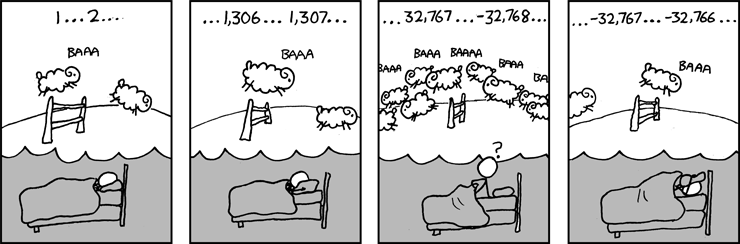
\includegraphics{xkcd.png} \\
    \footnotesize\sffamily%
    Tiré de \href{http://xkcd.com/571/}{XKCD.com}
  \end{minipage}
  \setkeys{Gin}{width=0.8\textwidth}
\end{vplace}

\mainmatter

\chapter{Arithmétique des ordinateurs}
\label{chap:ordinateurs}

%%%
%%% Fichers de solutions et de réponses
%%%

\Opensolutionfile{reponses}[reponses-arithmetique_ordinateurs]
\Opensolutionfile{solutions}[solutions-arithmetique_ordinateurs]

\begin{Filesave}{reponses}
\bigskip
\section*{Réponses}

\noindent
La notation $x_{b}$ signifie que le nombre $x$ est en base $b$. On
omet généralement $b$ pour les nombres en base 10.

\end{Filesave}

\begin{Filesave}{solutions}
\section*{Chapitre \ref{chap:ordinateurs}}
\addcontentsline{toc}{section}{Chapitre \protect\ref{chap:ordinateurs}}

\noindent
La notation $x_{b}$ signifie que le nombre $x$ est en base $b$. On
omet généralement $b$ pour les nombres en base 10.

\end{Filesave}

%%%
%%% Début des exercices
%%%

\begin{exercice}
  Convertir les nombres décimaux suivants en base 6, puis en binaire.
  \begin{enumerate}
  \item 119
  \item 343
  \item 96
  \item 43
  \end{enumerate}
  \begin{sol}
    L'algorithme de conversion des nombres décimaux en une base $b$ se
    résume essentiellement à ceci pour la partie entière:
    \begin{enumerate}[1.]
    \item les chiffres du nombre en base $b$ sont obtenus de droite à
      gauche en prenant le reste de divisions par $b$;
    \item on divise par $b$ d'abord le nombre décimal d'origine, puis
      la partie entière de la division précédente, jusqu'à ce que
      celle-ci soit égale à 0.
    \end{enumerate}
    On a donc les résultats suivants.
    \begin{enumerate}
    \item
      \begin{minipage}[t]{0.48\linewidth}
        Conversion en base 6:
        \begin{align*}
          119 \div 6 &= 19 \text{ reste } 5 \\
           19 \div 6 &= 3 \text{ reste } 1 \\
            3 \div 6 &= 0 \text{ reste } 3,
        \end{align*}
        d'où $119 \equiv 315_6$.
      \end{minipage}
      \hfill
      \begin{minipage}[t]{0.48\linewidth}
        Conversion en binaire:
        \begin{align*}
          119 \div 2 &= 59 \text{ reste } 1 \\
           59 \div 2 &= 29 \text{ reste } 1 \\
           29 \div 2 &= 14 \text{ reste } 1 \\
           14 \div 2 &= 7 \text{ reste } 0 \\
            7 \div 2 &= 3 \text{ reste } 1 \\
            3 \div 2 &= 1 \text{ reste } 1 \\
            1 \div 2 &= 0 \text{ reste } 1,
        \end{align*}
        d'où $119 \equiv 1110111_2$.
      \end{minipage}
    \item
      \begin{minipage}[t]{0.48\linewidth}
        Conversion en base 6:
        \begin{align*}
          343 \div 6 &= 57 \text{ reste } 1 \\
           57 \div 6 &= 9 \text{ reste } 3 \\
            9 \div 6 &= 1 \text{ reste } 3 \\
            1 \div 6 &= 0 \text{ reste } 1,
        \end{align*}
        d'où $343 \equiv 1331_6$.
      \end{minipage}
      \hfill
      \begin{minipage}[t]{0.48\linewidth}
        Conversion en binaire:
        \begin{align*}
          343 \div 2 &= 171 \text{ reste } 1 \\
          171 \div 2 &= 85 \text{ reste } 1 \\
           85 \div 2 &= 42 \text{ reste } 1 \\
           42 \div 2 &= 21 \text{ reste } 0 \\
           21 \div 2 &= 10 \text{ reste } 1 \\
           10 \div 2 &= 5 \text{ reste } 0 \\
            5 \div 2 &= 2 \text{ reste } 1 \\
            2 \div 2 &= 1 \text{ reste } 0 \\
            1 \div 2 &= 0 \text{ reste } 1,
        \end{align*}
        d'où $119 \equiv 101010111_2$.
      \end{minipage}
    \item
      \begin{minipage}[t]{0.48\linewidth}
        Conversion en base 6:
        \begin{align*}
          96 \div 6 &= 16 \text{ reste } 0 \\
          16 \div 6 &= 2 \text{ reste } 4 \\
           2 \div 6 &= 0 \text{ reste } 2,
        \end{align*}
        d'où $96 \equiv 240_6$.
      \end{minipage}
      \hfill
      \begin{minipage}[t]{0.48\linewidth}
        Conversion en binaire:
        \begin{align*}
          96 \div 2 &= 48 \text{ reste } 0 \\
          48 \div 2 &= 24 \text{ reste } 0 \\
          24 \div 2 &= 12 \text{ reste } 0 \\
          12 \div 2 &= 6 \text{ reste } 0 \\
           6 \div 2 &= 3 \text{ reste } 0 \\
           3 \div 2 &= 1 \text{ reste } 1 \\
           1 \div 2 &= 0 \text{ reste } 1,
        \end{align*}
        d'où $96 \equiv 1100000_2$.
      \end{minipage}
    \item
      \begin{minipage}[t]{0.48\linewidth}
        Conversion en base 6:
        \begin{align*}
          43 \div 6 &= 7 \text{ reste } 1 \\
           7 \div 6 &= 1 \text{ reste } 1 \\
           1 \div 6 &= 0 \text{ reste } 1,
        \end{align*}
        d'où $43 \equiv 111_6$.
      \end{minipage}
      \hfill
      \begin{minipage}[t]{0.48\linewidth}
        Conversion en binaire:
        \begin{align*}
          43 \div 2 &= 21 \text{ reste } 1 \\
          21 \div 2 &= 10 \text{ reste } 1 \\
          10 \div 2 &= 5 \text{ reste } 0 \\
           5 \div 2 &= 2 \text{ reste } 1 \\
           2 \div 2 &= 1 \text{ reste } 0 \\
           1 \div 2 &= 0 \text{ reste } 1,
        \end{align*}
        d'où $43 \equiv 101011_2$.
      \end{minipage}
    \end{enumerate}
  \end{sol}
  \begin{rep}
    \begin{enumerate}
    \item $315_6$, $1110111_2$
    \item $1331_6$, $101010111_2$
    \item $240_6$, $1100000_2$
    \item $111_6$, $101011_2$
    \end{enumerate}
  \end{rep}
\end{exercice}

\begin{exercice}
  Convertir les nombres hexadécimaux suivants en nombres décimaux.
  \begin{enumerate}
  \item A1B
  \item 12A
  \item B41
  \item BAFFE
  \end{enumerate}
  \begin{sol}
    On fait les deux premières conversions à l'aide de la définition
    d'un nombre hexadécimal, puis les deux dernières à l'aide de
    l'algorithme de conversion des nombres en base $b$ vers la base
    10.
    \begin{enumerate}
    \item $\text{A1B}_{16} = 10 \times 16^2 + 1 \times 16 + 11 = \nombre{2587}$
    \item $\text{12A}_{16} = 1 \times 16^2 + 2 \times 16 + 10 = 298$
    \item $\text{B41}_{16} = (11 \times 16 + 4) \times 16 + 1 = \nombre{2881}$
    \item $\text{BAFFE}_{16} = ((((11 \times 16 + 10) \times 16) + 15)
      \times 16) + 15) \times  + 14 = \nombre{765950}$
    \end{enumerate}
  \end{sol}
  \begin{rep}
    \begin{inparaenum}
    \item \nombre{2587}
    \item 298
    \item \nombre{2881}
    \item \nombre{765950}
    \end{inparaenum}
  \end{rep}
\end{exercice}

\begin{exercice}
  \begin{enumerate}
  \item Utiliser l'algorithme de conversion des nombres en base $b$
    vers la base 10 et les idées de l'exemple 4.6 des notes de cours
    pour trouver une formule générale donnant la position de l'élément
    $a_{ijk}$ d'un tableau de dimensions $I \times J \times K$ dans
    l'ordre de la liste des éléments du tableau. Utiliser l'ordre
    lexicographique, où le tableau est rempli dans l'ordre $a_{111},
    a_{112}, \dots, a_{11K}, a_{121}, a_{122}, \dots$
  \item Répéter la partie a) en utilisant l'ordre S, où le tableau
    est plutôt rempli dans l'ordre $a_{111}, a_{211}, \dots, a_{I11},
    a_{121}, a_{221}, \dots$.  Comparer la réponse avec celle de
    l'exercice 3.7~b) de \cite{Goulet_intro_S}.
  \end{enumerate}
  \begin{sol}
    La généralisation de l'algorithme de conversion des nombres en
    base $b$ vers la base 10 à la conversion d'un nombre
    \begin{displaymath}
      x = x_{m-1}x_{m-2} \cdots x_1x_0
    \end{displaymath}
    en base $[b_{m-1}\; \dots\; b_0]$ vers la base 10 est la suivante
    (nombre entiers seulement):
    \begin{enumerate}[1.]
    \item Poser $x = 0$.
    \item Pour $i = m - 1, m - 2, \dots, 0$, faire les étapes suivantes.
      \begin{enumerate}
      \item Trouver $d_i$, le nombre décimal correspondant au symbole
        $x_i$.
      \item Poser $x = x b_{i - 1} + d_i$, avec $b_{-1} = 1$.
      \end{enumerate}
    \end{enumerate}
    Cet algorithme permet de trouver les formules demandées.
    \begin{enumerate}
    \item Tel que présenté à l'exemple 4.6 des notes de cours, on
      trouve la position de l'élément $a_{ijk}$ dans l'ordre de la
      liste des éléments du tableau en convertissant le nombre $[i -
      1\; j - 1\; k - 1]$ de la base $[I\; J\; K]$ à la base 10, puis
      à additionnant 1. À l'aide de l'algorithme ci-dessus, on obtient
      \begin{displaymath}
        [((i - 1) \times J + j - 1) \times K + k - 1] + 1
        = k + K (j - 1 + J (i - 1))
      \end{displaymath}
    \item Dans l'ordre S, on convertit le nombre $[k - 1\; j - 1\; i -
      1]$ exprimé dans la base $[K\; J\; I]$ en base 10. On obtient alors
      \begin{displaymath}
        [((k - 1) \times J + j - 1) \times I + i - 1] + 1
        = i + I (j - 1 + J (k - 1))
      \end{displaymath}
      soit la même réponse qu'à l'exercice 3.7~b) de
      \cite{Goulet_intro_S}.
    \end{enumerate}
  \end{sol}
  \begin{rep}
    \begin{enumerate}
    \item $k + K (j - 1 + J (i - 1))$
    \item $i + I (j - 1 + J (k - 1))$
    \end{enumerate}
  \end{rep}
\end{exercice}

\begin{exercice}
  La norme IEEE~754 pour les nombres en virgule flottante $(S,
  E, F)$ en simple précision est le suivant:
  \begin{itemize}
  \item longueur totale de $m = 32$ bits;
  \item 1 bit pour le signe $S$ (valeur de 0 pour un nombre positif);
  \item 8 bits pour l'exposant $E$, avec un biais de 127;
  \item 23 bits pour la partie fractionnaire $F$.
  \end{itemize}
  Un nombre $x$ est donc représenté comme
  \begin{displaymath}
    x = (-1)^S \times 2^{E - 127} \times 1,F.
  \end{displaymath}
  Trouver les valeurs $\varepsilon$, $x_{\max}$ et $x_{\min}$ pour les
  nombres en simple précision. Comparer les résultats avec les limites
  du type \texttt{Single} en VBA.
  \begin{sol}
    Voir les notes de cours de la section 4.4. Les calculs sont
    exactement les mêmes que pour les nombres en double précision.
  \end{sol}
  \begin{rep}
    $\varepsilon = 2^{-23} = 1,192 \times 10^{-7}$,
    $x_{\max} = (2 - 2^{-23}) \times 2^{127} = 3,403 \times 10^{38}$,
    $x_{\min} = 2^{-126} = 1,175 \times 10^{-38}$ (nombre normal) ou
    $x_{\min} = 2^{-149} = 1,401 \times 10^{-45}$ (nombre sous-normal)
  \end{rep}
\end{exercice}

\begin{exercice}
  Outre les types \texttt{Single} et \texttt{Double} pour représenter
  des nombres en virgule flottante, le VBA dispose également des types
  \texttt{Integer}, \texttt{Long} et \texttt{Byte} pour représenter
  des nombres entiers. Comme son nom l'indique, le type \texttt{Byte}
  utilise huit bits d'espace mémoire et ne sert que pour les entiers
  positifs. Les types \texttt{Integer} et \texttt{Long} requièrent 16
  et 32 bits, respectivement, et peuvent contenir des nombres
  négatifs. En supposant qu'un bit est réservé pour le signe dans ces
  deux derniers types (ce qui n'est pas exactement le cas), trouver le
  plus grand nombre admissible pour chaque type de données.
  \begin{sol}
    L'étendue des nombres admissibles pour le type \texttt{Byte} est
    $[0, 2^8 - 1] = [0, 255]$. Les nombres maximaux pour les types
    \texttt{Integer} et \texttt{Long} sont, respectivement, $2^{15} -
    1 = \nombre{32767}$ et $2^{31} - 1 = \nombre{2147483647}$.
    L'étendue est plus grande de 1 pour les nombres négatifs
    ($-\nombre{32768}$ et $-\nombre{2147483648}$) parce que les
    nombres sont en fait stockés en compléement à deux; voir
    \url{http://fr.wikipedia.org/wiki/Complément_à_deux}.
  \end{sol}
  \begin{rep}
    Type \texttt{Byte}: 255; type \texttt{Integer}: \nombre{32767};
    type \texttt{Long}: \nombre{2147483647}.
  \end{rep}
\end{exercice}

\begin{exercice}
  Représenter les nombres suivants comme des nombres en virgule
  flottante en simple précision selon la norme IEEE~754.
  \begin{enumerate}
  \item $-\nombre{1234}$
  \item 55
  \item \nombre{8191}
  \item $-10$
  \item $\frac{2}{3}$
  \item $\frac{1}{100}$
  \end{enumerate}
  \begin{sol}
    Dans les égalités ci-dessous, le côté droit est en binaire.
    \begin{enumerate}
    \item Premièrement, $1234 \equiv 10011010010_2$. On a donc
      \begin{align*}
        -\nombre{1234}
        &= (-1)^1 \times 2^{10} \times 1,001101001 \\
        &= (-1)^1 \times 2^{137 - 127} \times 1,1010010.
      \end{align*}
      Or, puisque $137 \equiv 10001001_2$, on a la représentation en
      simple précision
      \begin{displaymath}
        \ieee{1}{10001001}{00110100100000000000000}
      \end{displaymath}
    \item On a $55 \equiv 110111_2$, d'où
      \begin{align*}
        55
        &= (-1)^0 \times 2^5 \times 1,10111 \\
        &= (-1)^0 \times 2^{132 - 127} \times 1,10111.
      \end{align*}
      Or, puisque $132 \equiv 10000100_2$, on a la représentation en
      simple précision
      \begin{displaymath}
        \ieee{0}{10000100}{10111000000000000000000}
      \end{displaymath}
    \item On a $\nombre{8191} \equiv 1111111111111_2$ et $149 \equiv
      10001011$, d'où
      \begin{align*}
        \nombre{8191}
        &= (-1)^0 \times 2^{12} \times 1,111111111111 \\
        &= (-1)^0 \times 2^{149 - 127} \times 1,111111111111 \\
        &= \ieee{0}{10001011}{11111111111100000000000}.
      \end{align*}
    \item On a $10 \equiv 1010_2$ et $130 \equiv
      10000010$, d'où
      \begin{align*}
        -10
        &= (-1)^1 \times 2^3 \times 1,010 \\
        &= (-1)^1 \times 2^{130 - 127} \times 1,010 \\
        &= \ieee{1}{10000010}{01000000000000000000000}.
      \end{align*}
    \item La représentation de $\frac{2}{3}$ en binaire est
      $0,101010\dots$. (La façon la plus simple d'obtenir ce résultat
      consiste à convertir $\frac{2}{3} \times 2^n$, où $n$ est le
      nombre de bits souhaité après la virgule). Puisque $126 \equiv
      1111110_2$, on a
      \begin{align*}
        \frac{2}{3}
        &= (-1)^0 \times 2^{-1} \times 1,01010101010101010101010 \\
        &= (-1)^0 \times 2^{126 - 127} \times 1,01010101010101010101010 \\
        &= \ieee{0}{01111110}{01010101010101010101010}.
      \end{align*}
    \item La représentation binaire de $\frac{1}{100}$ est infinie:
      $0,000000101000111101\dots$. Puisque $120 \equiv 01111000_2$, on
      a
      \begin{align*}
        \frac{1}{100}
        &= (-1)^0 \times 2^{-7} \times 1,01000111101011100001010 \\
        &= (-1)^0 \times 2^{120 - 127} \times 1,01000111101011100001010 \\
        &= \ieee{0}{01111000}{01000111101011100001010}
      \end{align*}
    \end{enumerate}
  \end{sol}
  \begin{rep}
    \begin{enumerate}
    \item \ieee{1}{10001001}{00110100100000000000000}
    \item \ieee{0}{10000100}{10111000000000000000000}
    \item \ieee{0}{10001011}{11111111111100000000000}
    \item \ieee{1}{10000010}{01000000000000000000000}
    \item \ieee{0}{01111110}{01010101010101010101010}
    \item \ieee{0}{01111000}{01000111101011100001010}
    \end{enumerate}
  \end{rep}
\end{exercice}

\begin{exercice}
  \label{ex:ordinateurs:ieee}
  Les nombres ci-dessous sont représentés en format binaire selon la
  norme IEEE~754 pour les nombres en simple précision. Convertir ces
  nombres en décimal.
  \begin{enumerate}
  \item \ieee{0}{00111101}{10010000100000000000000}
  \item \ieee{1}{00111101}{10010000100000000000000}
  \item \ieee{0}{10000100}{10010000100000000000000}
  \item \ieee{1}{10000100}{10010000100000000000000}
  \end{enumerate}
  \begin{sol}
    \begin{enumerate}
    \item Puisque $111101_2 \equiv 61$, on a le nombre
      \begin{align*}
        (-1)^0 \times 2^{61 - 127} \times 1,100100001
        &= (-1)^0 \times 2^{-66} \times 1,100100001 \\
        &= 2^{-66} (1 + 2^{-1} + 2^{-4} + 2^{-9}) \\
        &\equiv \nombre{2,120229346} \times 10^{-20}.
      \end{align*}
    \item Signe inversé par rapport à la partie a).
    \item Puisque $10000100_2 = 2^7 + 2^2 \equiv 132$, on a le nombre
      \begin{align*}
        (-1)^0 \times 2^{132 - 127} \times 1,100100001
        &= (-1)^0 \times 2^5 \times 1,100100001 \\
        &= 2^5 (1 + 2^{-1} + 2^{-4} + 2^{-9}) \\
        &\equiv \nombre{50,0625}.
      \end{align*}
    \item Signe inversé par rapport à la partie c).
    \end{enumerate}
  \end{sol}
  \begin{rep}
    \sloppy
    \begin{inparaenum}
    \item $\nombre{2,120229346} \times 10^{-20}$
    \item $\nombre{-2,120229346} \times 10^{-20}$
    \item $50,0625$
    \item $-50,0625$
    \end{inparaenum}
  \end{rep}
\end{exercice}

\begin{exercice}
  Trouver, pour les nombres des parties a) et c) de l'exercice
  \ref{chap:ordinateurs}.\ref{ex:ordinateurs:ieee}, le nombre suivant
  et le nombre précédent en représentation binaire.
  \begin{sol}
    \begin{enumerate}
    \item Le nombre suivant est
      \begin{displaymath}
        \ieee{0}{00111101}{10010000100000000000001},
      \end{displaymath}
      soit
      \begin{displaymath}
        2^{-66} (1 + 2^{-1} + 2^{-4} + 2^{-9} + 2^{-23}) \\
        \equiv \nombre{2,120229508} \times 10^{-20}.
      \end{displaymath}
      Le nombre précédent est
      \begin{displaymath}
        \ieee{0}{00111101}{10010000011111111111111},
      \end{displaymath}
      soit
      \begin{displaymath}
        2^{-66} (1 + 2^{-1} + 2^{-4} + 2^{-9} - 2^{-23}) \\
        \equiv \nombre{2,120229185} \times 10^{-20}.
      \end{displaymath}
      \stepcounter{enumi}
    \item Le nombre suivant est
      \begin{displaymath}
        \ieee{0}{10000100}{10010000100000000000001},
      \end{displaymath}
      soit
      \begin{displaymath}
        2^5 (1 + 2^{-1} + 2^{-4} + 2^{-9} + 2^{-23}) \\
        \equiv \nombre{50,062503815}.
      \end{displaymath}
      Le nombre précédent est
      \begin{displaymath}
        \ieee{0}{10000100}{10010000011111111111111},
      \end{displaymath}
      soit
      \begin{displaymath}
        2^5 (1 + 2^{-1} + 2^{-4} + 2^{-9} - 2^{-23}) \\
        \equiv \nombre{50,062496185}.
      \end{displaymath}
      On remarque que les nombres sont beaucoup plus éloignés les uns
      des autres ici qu'en a).
    \end{enumerate}
  \end{sol}
  \begin{rep}
    \begin{inparaenum}
    \item $\nombre{2,120229508} \times 10^{-20}$ et
      $\nombre{2,120229185} \times 10^{-20}$
      \stepcounter{enumi}
    \item $\nombre{50,062503815}$ et $\nombre{50,062496185}$
    \end{inparaenum}
  \end{rep}
\end{exercice}

\Closesolutionfile{reponses}
\Closesolutionfile{solutions}

%%%
%%% Insérer les réponses
%%%
\input{reponses-arithmetique_ordinateurs}


%%% Local Variables:
%%% mode: latex
%%% TeX-master: "exercices_methodes_numeriques"
%%% End:

\include{resolution_equations}
\include{integration_numerique}

\appendix
%%% Copyright (C) 2018 Vincent Goulet
%%%
%%% Ce fichier fait partie du projet
%%% «Méthodes numériques en actuariat avec R»
%%% http://github.com/vigou3/methodes-numeriques-en-actuariat
%%%
%%% Cette création est mise à disposition selon le contrat
%%% Attribution-Partage dans les mêmes conditions 4.0
%%% International de Creative Commons.
%%% http://creativecommons.org/licenses/by-sa/4.0/

\chapter{Solutions des exercices}
\label{chap:solutions}
\markboth{Solutions des exercices}{Solutions des exercices}

\begingroup

%% Environnement Schunk simplifié pour l'affichage des réponses
\renewenvironment{Schunk}{%
  \setlength{\topsep}{0pt}
  \colorlet{shadecolor}{codebg}
  \begin{snugshade*}}%
  {\end{snugshade*}}
\input{solutions-generation}
\input{solutions-simulation}
\input{solutions-montecarlo}

\endgroup

%%% Local Variables:
%%% mode: latex
%%% TeX-engine: xetex
%%% TeX-master: "methodes-numeriques-en-actuariat_simulation"
%%% coding: utf-8
%%% End:


\bibliography{r,math,stat,informatique,vg}

\cleartoverso
\thispagestyle{empty}
\vspace*{\fill}

\begingroup
\calccentering{\unitlength}
\begin{adjustwidth*}{\unitlength}{-\unitlength}
  \begin{flushleft}
    \small %
    Ce document a été produit avec le système de mise en page
    {\XeLaTeX}. Le texte principal est en Lucida Bright~OT 11~points,
    les mathématiques en Lucida Bright Math~OT, le code informatique
    en Lucida Grande Mono~DK et les titres en Adobe Myriad~Pro. Des
    icônes proviennent de la police Font~Awesome. Les graphiques ont
    été réalisés avec R.
  \end{flushleft}
\end{adjustwidth*}
\endgroup
\vfill


\cleartoverso
%%% Copyright (C) 2018 Vincent Goulet
%%%
%%% Ce fichier fait partie du projet
%%% «Méthodes numériques en actuariat avec R»
%%% http://github.com/vigou3/methodes-numeriques-en-actuariat
%%%
%%% Cette création est mise à disposition selon le contrat
%%% Attribution-Partage dans les mêmes conditions 4.0
%%% International de Creative Commons.
%%% http://creativecommons.org/licenses/by-sa/4.0/

\begingroup

\TPGrid{3}{36}
\textblockorigin{0mm}{0mm}
\setlength{\parindent}{0mm}
\setlength{\banderougewidth}{2\TPHorizModule}
\setlength{\bandeorwidth}{\TPHorizModule}
\setlength{\gapwidth}{2pt}
\addtolength{\bandeorwidth}{-\gapwidth}

%% bandeau identitaire arrière
\begin{textblock*}{8.5in}[0,1](0mm,30\TPVertModule)
  \textcolor{or}{\rule{\bandeorwidth}{\TPVertModule}}%      % bande or
  \rule{\gapwidth}{0pt}%                                    % filet
  \textcolor{rouge}{\rule{\banderougewidth}{\TPVertModule}} % bande rouge
\end{textblock*}

% code-barre
% \begin{textblock*}{0.9\TPHorizModule}(0.1\TPHorizModule,25\TPVertModule)
%   \includegraphics[height=4\TPVertModule]{codebarre_\ISBN}
% \end{textblock*}

\endgroup


\end{document}

%%% Local Variables:
%%% mode: latex
%%% TeX-engine: xetex
%%% TeX-master: t
%%% coding: utf-8
%%% End:
